{\setbeamerfont{framesubtitle}{size=\tiny}
\begin{frame}{\fe{Exercice 4 : contact thermo mécanique}
                 {Exercise 4: thermo mechanicla contact}}
             {\url{https://www-cast3m.cea.fr/index.php?page=exemples&exemple=formation_pasapas_4_initial}}
  \small
  \begin{itemize}
    \item \fe{Dilatation thermique de 2 barreaux et mise en contact}
             {Thermal expansion of 2 bars and coming into contact}
  \end{itemize}
  \begin{center}
    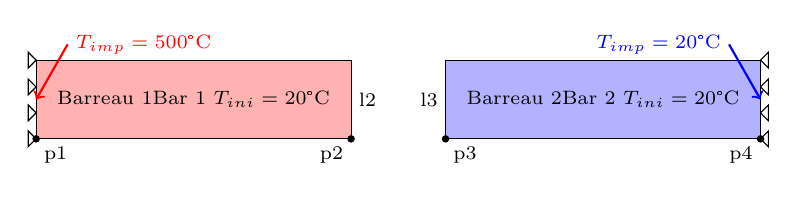
\begin{tikzpicture}
      \scriptsize
      \def\lbar{4}  \def\hbar{1}   \def\gap{1.2}
      \draw [-] (0,0)          -- (-0.1,-0.1)           -- (-0.1,0.1)            --cycle;
      \draw [-] (0,0.33*\hbar) -- (-0.1,0.33*\hbar-0.1) -- (-0.1,0.33*\hbar+0.1) --cycle;
      \draw [-] (0,0.66*\hbar) -- (-0.1,0.66*\hbar-0.1) -- (-0.1,0.66*\hbar+0.1) --cycle;
      \draw [-] (0,\hbar)      -- (-0.1,\hbar-0.1)      -- (-0.1,\hbar+0.1)      --cycle;
      \draw[fill=red!30] (0,0) rectangle (\lbar,\hbar);
      \filldraw (0,0)     circle(0.4mm) node[anchor=north west] {\kw{p1}};
      \filldraw (\lbar,0) circle(0.4mm) node[anchor=north east] {\kw{p2}};
      \draw (\lbar,0.5*\hbar) node[anchor=west] {\kw{l2}};
      \draw (0.5*\lbar,0.5*\hbar) node {\fe{Barreau 1}{Bar 1} \red{$T_{\tx{ini}}=20$°C}};
      \draw [->,thick,red] (0.4,\hbar+0.2) node[anchor=west] {$T_{\tx{imp}}=500$°C} -- (0,0.5*\hbar);
      \draw [-] (2*\lbar+\gap,0)          -- (2*\lbar+\gap+0.1,-0.1)           -- (2*\lbar+\gap+0.1,0.1)            --cycle;
      \draw [-] (2*\lbar+\gap,0.33*\hbar) -- (2*\lbar+\gap+0.1,0.33*\hbar-0.1) -- (2*\lbar+\gap+0.1,0.33*\hbar+0.1) --cycle;
      \draw [-] (2*\lbar+\gap,0.66*\hbar) -- (2*\lbar+\gap+0.1,0.66*\hbar-0.1) -- (2*\lbar+\gap+0.1,0.66*\hbar+0.1) --cycle;
      \draw [-] (2*\lbar+\gap,\hbar)      -- (2*\lbar+\gap+0.1,\hbar-0.1)      -- (2*\lbar+\gap+0.1,\hbar+0.1)      --cycle;
      \draw[fill=blue!30] (\lbar+\gap,0) rectangle (2*\lbar+\gap,\hbar);
      \filldraw (\lbar+\gap,0)   circle(0.4mm) node[anchor=north west] {\kw{p3}};
      \filldraw (2*\lbar+\gap,0) circle(0.4mm) node[anchor=north east] {\kw{p4}};
      \draw (\lbar+\gap,0.5*\hbar) node[anchor=east] {\kw{l3}};
      \draw (1.5*\lbar+\gap,0.5*\hbar) node {\fe{Barreau 2}{Bar 2} \blue{$T_{\tx{ini}}=20$°C}};
      \draw [->,thick,blue] (2*\lbar+\gap-0.4,\hbar+0.2) node[anchor=east] {$T_{\tx{imp}}=20$°C} -- (2*\lbar+\gap,0.5*\hbar);
    \end{tikzpicture}
  \end{center}
  \begin{itemize}
    \item<2-> \fe{\green{Objectif : ajouter le \g{contact thermique} entre \kw{l2} et \kw{l3},\\
                        \qquad \qquad ~ c'est à dire le transfert de chaleur lors du contact.}}
                {\green{Purpose: add \g{thermal contact} between \kw{l2} and \kw{l3},\\
                        \qquad \qquad this means the heat transfer when contact takes place.}}\\
    \begin{center}
      \fe{\avous{~À vous de jouer !}}{\avous{~It's up to you!}}
    \end{center}
  \end{itemize}
\end{frame}
}

{\setbeamerfont{framesubtitle}{size=\tiny}
\begin{frame}{\fe{Exercice 4 : contact thermo mécanique}
                 {Exercise 4: thermo mechanicla contact}}
             {\url{https://www-cast3m.cea.fr/index.php?page=exemples&exemple=formation_pasapas_4_initial}}
  \begin{itemize}
    \item \fe{Quelques objets utiles}{Some useful objects}\\
    \footnotesize
    \kw{p2 p2} \fe{points à gauche et à droite du jeu}{points on the left/right of the gap}\\
    \kw{p3 l3} \fe{lignes à gauche et droite du jeu}{lines on the left/right of the gap}\\
    \normalsize
    \item \fe{Quelques opérateurs utiles}{Some useful operators}\\
    \footnotesize
    \kwr{COOR} \fe{obtenir les coordonnées de points}{get points coordinates}\\
    \kwr{RELA} \fe{imposer linéaire entre degrés de liberté}{impose a linear relation between degrees of freedom}\\
    \normalsize
    \item \fe{Quelques indices utiles de la table}{Some useful table indices}\\
    \footnotesize
    \kwg{'WTABLE'.'BLOCAGES\_THERMIQUES'} \fe{CL thermiques courrantes}{current thermal BC}\\
    \normalsize
  \end{itemize}
\end{frame}
}

\begin{frame}{\fe{Exercice 4 : contact thermo mécanique}
                 {Exercise 4: thermo mechanicla contact}}
             {\fe{Solution avec REEV\_MEC}{Solution with REEV\_MEC}}
  \footnotesize
  \begin{itemize}
    \small
    \item \fe{Utiliser la \red{boucle de convergence thermo mécanique}}{Use the \red{thermo mechanical convergence loop}}
    \item \fe{Créer une \kwr{RELA}tion entre les températures de \kw{l2} et \kw{l3}}
             {Create a \kwr{RELA}tion between temperatures at \kw{l2} and \kw{l3}}
    \item \fe{Utiliser la procédure \kwv{REEV\_MEC}}{Use procedure \kwv{REEV\_MEC}}
    \item \fe{Calculer le jeu à l'itération courante et modifier (ou non) l'indice \kwg{'WTABLE'.'BLOCAGES\_THERMIQUE'}}
             {Calculate the gap at current iteration and modifiy \kwg{'WTABLE'.'BLOCAGES\_THERMIQUE'} or not}
  \end{itemize}
  \vspace{4.5cm}
  \scriptsize
  \begin{textblock*}{10cm}(0.3cm,-4cm)
    \fe{\emph{Programme principal}}{\emph{Main program}}
%    \lstinputlisting[basicstyle=\ttfamily\tiny, language=gibiane, firstline=49, lastline=52]{dgibi/formation_pasapas_4_solution.dgibi}
  \end{textblock*}
  \begin{textblock*}{10cm}(6.cm,-4cm)
    \fe{\emph{\violet{Procédure REEV\_MEC}}}{\emph{\violet{REEV\_MEC procedure}}}
%    \lstinputlisting[basicstyle=\ttfamily\tiny, language=gibiane, firstline=67, lastline=81]{dgibi/formation_pasapas_4_solution.dgibi}
  \end{textblock*}
\end{frame}

\begin{frame}{\fe{Exercice 4 : contact thermo mécanique}
                 {Exercise 4: thermo mechanicla contact}}
             {\fe{Solution avec REEV\_MEC}{Solution with REEV\_MEC}}
  \begin{itemize}
    \item \fe{Résultats}{Results}\\
    \vspace{5cm}
  \end{itemize}
\end{frame}
